\subsection{Okna potomne}

\subsubsection{Tworzenie okien potomnych}

Główne okno aplikacji, jak również każde kolejne okno z którym styka się użytkownik,
zwykle posiada jakieś okna potomne (zwane inaczej {\em kontrolkami}), za pomocą których
użytkownik mógłby komunikować się z aplikacją.

Dwa najprostsze rodzaje okien potomnych to pole tekstowe i przycisk. Okazuje się jednak, że 
klasa okna (na przykład klasa {\bf BUTTON} definiująca przyciski), tak naprawdę definiuje nie {\em jeden} typ
okna potomnego, ale całą rodzinę okien potomnych, różniących się właściwościami. Odpowiedni styl
okna podaje się jako jeden z parametrów do funkcji {\bf CreateWindow}.

Zobaczmy prosty przykład tworzenia okien potomnych o różnych stylach:

\begin{scriptsize}
\begin{verbatim}
/*
 *
 * Tworzenie okien potomnych
 *
 */
#include <windows.h>
#include <string.h>

/* Deklaracja wyprzedzająca: funkcja obsługi okna */
LRESULT CALLBACK WindowProcedure(HWND, UINT, WPARAM, LPARAM);
/* Nazwa klasy okna */
char szClassName[] = "PRZYKLAD";

struct
{
     TCHAR * szClass;
     int     iStyle ;
     TCHAR * szText ;
} button[] =
{
     "BUTTON"  , BS_PUSHBUTTON    ,  "PUSHBUTTON",
     "BUTTON"  , BS_AUTOCHECKBOX  ,  "CHECKBOX",
     "BUTTON"  , BS_RADIOBUTTON   ,  "RADIOBUTTON",
     "BUTTON"  , BS_GROUPBOX      ,  "GROUPBOX",
     "EDIT"    , WS_BORDER        ,  "TEXTBOX",
     "STATIC"  , WS_BORDER        ,  "STATIC",
} ;

#define NUM (sizeof button / sizeof button[0])

int WINAPI WinMain(HINSTANCE hThisInstance, HINSTANCE hPrevInstance, 
                   LPSTR lpszArgument, int nFunsterStil)
{
    HWND hwnd;               /* Uchwyt okna */
    MSG messages;            /* Komunikaty okna */
    WNDCLASSEX wincl;        /* Struktura klasy okna */

    /* Klasa okna */
    wincl.hInstance     = hThisInstance;
    wincl.lpszClassName = szClassName;
    wincl.lpfnWndProc   = WindowProcedure;    // wskaźnik na funkcję obsługi okna  
    wincl.style         = CS_DBLCLKS;                 
    wincl.cbSize        = sizeof(WNDCLASSEX);

    /* Domyślna ikona i wskaźnik myszy */
    wincl.hIcon   = LoadIcon(NULL, IDI_APPLICATION);
    wincl.hIconSm = LoadIcon(NULL, IDI_APPLICATION);
    wincl.hCursor = LoadCursor(NULL, IDC_ARROW);
    wincl.lpszMenuName = NULL; 
    wincl.cbClsExtra = 0;   
    wincl.cbWndExtra = 0;   
    /* Jasnoszare tło */
    wincl.hbrBackground = (HBRUSH)GetStockObject(LTGRAY_BRUSH);

    /* Rejestruj klasę okna */
    if(!RegisterClassEx(&wincl)) return 0;

    /* Twórz okno */
    hwnd = CreateWindowEx(
           0,                   
           szClassName,         
           "PRZYKLAD",       
           WS_OVERLAPPEDWINDOW, 
           CW_USEDEFAULT,       
           CW_USEDEFAULT,       
           CW_USEDEFAULT,       
           CW_USEDEFAULT,       
           HWND_DESKTOP,        
           NULL,                
           hThisInstance,       
           NULL                 
           );

    ShowWindow(hwnd, nFunsterStil);
    /* Pętla obsługi komunikatów */
    while(GetMessage(&messages, NULL, 0, 0))
    {
           /* Tłumacz kody rozszerzone */
           TranslateMessage(&messages);
           /* Obsłuż komunikat */
           DispatchMessage(&messages);
    }

    /* Zwróć parametr podany w PostQuitMessage( ) */
    return messages.wParam;
}

int xSize, ySize;

/* Tę funkcję woła DispatchMessage( ) */
LRESULT CALLBACK WindowProcedure(HWND hwnd, UINT message, 
                                 WPARAM wParam, LPARAM lParam)
{
    static HWND hwndButton[NUM];
    static int  cxChar, cyChar;  
    static      RECT r;
    HDC         hdc; 
    int         i;
    PAINTSTRUCT ps;

    TCHAR       szFormat[] = TEXT ("%-16s Akcja: %04X, ID:%04X, hWnd:%08X");
    TCHAR       szBuffer[80];
    
    switch (message)                  
    {
           case WM_CREATE :
                cxChar = LOWORD (GetDialogBaseUnits ()) ;
                cyChar = HIWORD (GetDialogBaseUnits ()) ;
                          
                for (i = 0 ; i < NUM ; i++)
                    hwndButton[i] = CreateWindow ( button[i].szClass, 
                                   button[i].szText,
                                   WS_CHILD | WS_VISIBLE | button[i].iStyle,
                                   cxChar, cyChar * (1 + 2 * i),
                                   20 * cxChar, 7 * cyChar / 4,
                                   hwnd, (HMENU) i,
                                   ((LPCREATESTRUCT) lParam)->hInstance, NULL) ;

              break;
           case WM_DESTROY:
              PostQuitMessage(0);        
              break;
           case WM_SIZE:
              xSize = LOWORD(lParam); 
              ySize = HIWORD(lParam); 
              
              r.left   = 24 * cxChar ;
              r.top    =  2 * cyChar ;
              r.right  = LOWORD (lParam) ;
              r.bottom = HIWORD (lParam) ;
              
              break;   
           case WM_COMMAND:
              hdc = GetDC (hwnd);
     
              ScrollWindow (hwnd, 0, -cyChar, &r, &r) ;              
              SelectObject (hdc, GetStockObject (SYSTEM_FIXED_FONT)) ;
          
              SetBkMode (hdc, TRANSPARENT) ;
              TextOut (hdc, 24 * cxChar, cyChar * (r.bottom / cyChar - 1),
                         szBuffer,
                         wsprintf (szBuffer, szFormat,
                         "WM_COMMAND",
                         HIWORD (wParam), LOWORD (wParam), lParam ));

              ReleaseDC( hwnd, hdc );                
              return DefWindowProc(hwnd, message, wParam, lParam);
           case WM_PAINT:
              hdc = BeginPaint (hwnd, &ps);  
              EndPaint( hwnd, &ps );
              break;   
              
           default:                   
              return DefWindowProc(hwnd, message, wParam, lParam);
    }
    return 0;
}
\end{verbatim}
\end{scriptsize}

\begin{figure}
\begin{center}
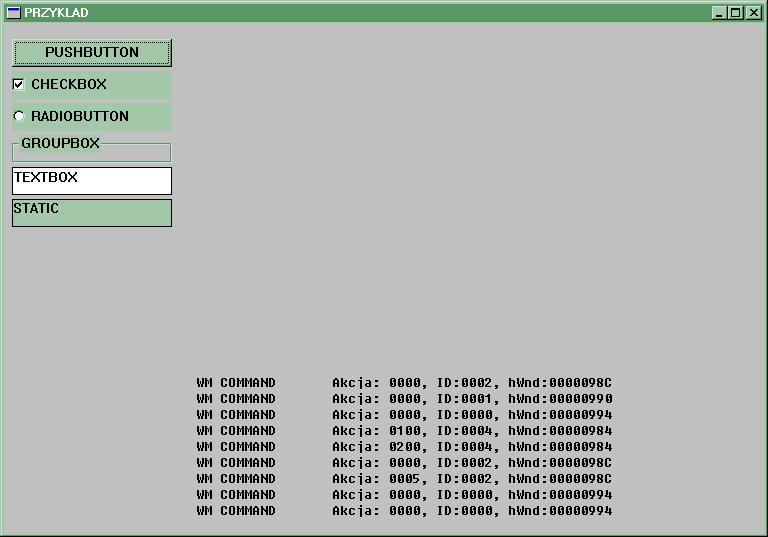
\includegraphics[width=0.75\textwidth]{./pic/p01}
\caption{Okna potomne komunikują się z oknem macierzystym za pomocą powiadomień}
\end{center}
\end{figure}

\subsubsection{Aktywowanie i deaktywowanie okien potomnych}

Programista może w każdej chwili uaktywnić bądź deaktywować okno\footnote{Okno potomne, które
jest nieaktywne zwykle ma szary kolor i nie przyjmuje fokusa.} za pomocą funkcji

\begin{scriptsize}
\begin{verbatim}
BOOL EnableWindow(

    HWND hWnd,	        // uchwyt okna
    BOOL bEnable 	// aktywacja bądź deaktywacja
   );
\end{verbatim}
\end{scriptsize}

\subsubsection{Komunikacja między oknem potomnym a macierzystym}

Komunikacja między oknem potomnym a oknem macierzystym odbywa się za pomocą
komunikatów przesyłanych między nimi. Komunikaty te pojawiają się w oknie macierzystym
jako WM\_COMMAND z dodatkowymi informacjami na temat powiadomienia od okna potomnego.

Spójrzmy przykładowo na powiadomienia, jakie oknu macierzystemu przysyła przycisk:
\begin{itemize}
	\item BN\_CLICKED : 0, przycisk został naciśnięty
	\item BN\_PAINT : 1, przycisk powinien zostać narysowany 
	\item BN\_PUSHED : 2, przycisk został wciśnięty
	\item BN\_UNPUSHED : 3, przycisk został wyciśnięty 
	\item BN\_DISABLE : 4, przycisk został deaktywowany
	\item BN\_DBLCLK : 5, przycisk został podwójnie naciśnięty
	\item BN\_SETFOCUS : 6, przycisk otrzymał fokusa
	\item BN\_KILLFOCUS : 7, przycisk stracił fokusa
\end{itemize}
 
Pole tekstowe przysyła oknu macierzystemu następujące powiadomienia:

\begin{itemize}
	\item EN\_SETFOCUS : 0x100, Pole tekstowe otrzymało fokusa
	\item EN\_KILLFOCUS : 0x200, Pole tekstowe straciłofokusa
	\item EN\_CHANGE : 0x300, Pole tekstowe zmieni zawartość
	\item EN\_UPDATE : 0x400, Pole tekstowe zmieniło zawartość
	\item EN\_ERRSPACE : 0x500, Pole tekstowe nie może zaallokować pamięci
	\item EN\_MAXTEXT : 0x501, Pole tekstowe przekroczyło rozmiar przy wskawianiu tekstu
	\item EN\_HSCROLL : 0x601, Pole tekstowe jest skrolowane w poziomie
	\item EN\_VSCROLL : 0x602, Pole tekstowe jest skrolowane w pionie
\end{itemize}

Okno główne może żądać od okien potomnych wykonania właściwych im operacji. Każda klasa okna
potomnego charakteryzuje się specyficznymi możliwościami. Okno główne wysyła do okien potomnych 
takie żądania za pomocą funkcji:

\begin{scriptsize}
\begin{verbatim}
LRESULT SendMessage(

    HWND hWnd,	// uchwyt okna
    UINT Msg,	// komunikat
    WPARAM wParam,	// parametr
    LPARAM lParam 	// parametr
   );
\end{verbatim}
\end{scriptsize}

Możliwości okien potomnych są naprawdę duże. Wspomnijmy tylko o kilku, natomiast pełna ich
lista dostępna jest w dokumentacji. Na przykład do pola tekstowego można wysłać komunikat:

\begin{scriptsize}
\begin{verbatim}
EM_FINDTEXT  
wParam = (WPARAM) (UINT) fuFlags; 
lParam = (LPARAM) (FINDTEXT FAR *) lpFindText;
\end{verbatim}
\end{scriptsize}

gdzie:
\begin{itemize}
	\item fuFlags : zero, FT\_MATCHCASE lub FT\_WHOLEWORD
	\item lpFindText : wskaźnik do struktury FINDTEXT zawierającej informacje o szukanym tekście
	\item wynik : -1 jeśli nie znaleziono tekstu, w przeciwnym razie indeks pozycji szukanego tekstu
\end{itemize}

oraz około 30 innych, odpowiadających m.in. za kolor, ograniczenie długości, przesuwanie zawartości, undo itd.

Do comboboxa można wysyłać komunikaty (łącznie około 20):
\begin{itemize}
	\item CB\_GETCOUNT : zwraca liczbę elementów
	\item CB\_FINDSTRING : szuka tekstu wśród elementów listy
	\item CB\_GETITEMDATA, CB\_SETITEMDATA : zwraca lub ustawia wartość związaną z elementem listy
	\item CB\_GETTOPINDEX, CB\_SETTOPINDEX : zwraca lub ustawia indeks pierwszego widocznego elementu listy
	\item $\ldots$
\end{itemize}

Do ListView można wysyłać komunikaty (łacznie około 30):
\begin{itemize}
	\item LVM\_DELETECOLUMN
	\item LVM\_ENSUREVISIBLE
	\item LVM\_GETCOLUMNWIDTH, LVM\_SETCOLUMNWIDTH
	\item LVM\_GETITEM, LVM\_SETITEM
	\item LVM\_SORTITEMS
	\item $\ldots$
\end{itemize}

Znając indentyfikator okna potomnego można łatwo uzyskać jego uchwyt i odwrotnie - znając
uchwyt można łatwo uzyskać identyfikator.

\begin{scriptsize}
\begin{verbatim}
id = GetDlgCtrlID (hwndChild) ;
hwndChild = GetDlgItem (hwndParent, id) ;
\end{verbatim}
\end{scriptsize}

Przykład użycia comboboxa:

\begin{scriptsize}
\begin{verbatim}
// Przygotuj kombo                   
hwndChild = CreateWindow ( "COMBOBOX", 
            "",
            WS_CHILD | WS_VISIBLE | CBS_DROPDOWNLIST,
            posX, posxY,
            width, height,
            hwnd, (HMENU) (1),
            ((LPCREATESTRUCT) lParam)->hInstance, NULL) ;
SendMessage( hwndChild, CB_ADDSTRING,     0, "Item1" );
SendMessage( hwndChild, CB_ADDSTRING,     0, "Item2" );
\end{verbatim}
\end{scriptsize}

\begin{figure}
\begin{center}
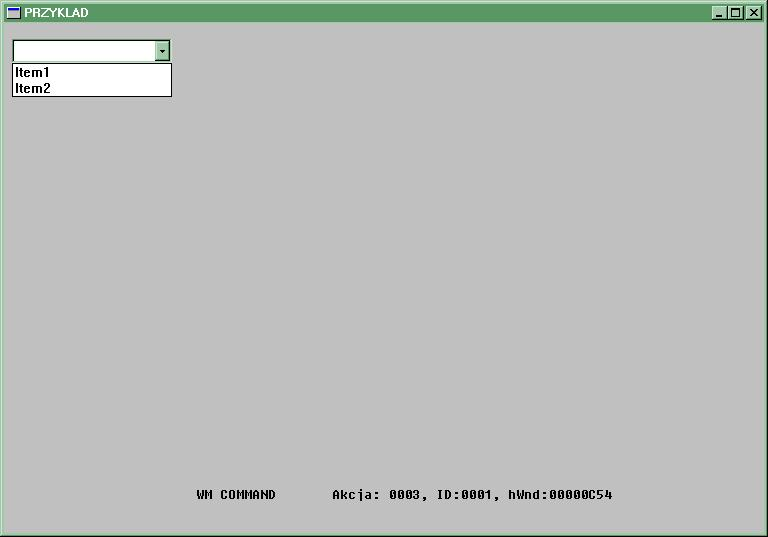
\includegraphics[width=0.75\textwidth]{./pic/p02}
\caption{Rozwijalny combobox z dwoma elementami}
\end{center}
\end{figure}

\subsection{Subclasowanie okien potomnych}

W poprzednich przykładach widzeliśmy, że okna potomne informują o zdarzeniach, które
zaszły w ich obszarze roboczym za pomocą powiadomień. Niestety, ilość możliwych
powiadomień przysyłanych przez okna potomne jest śmiesznie mała w porównaniu z
możliwościami jakie dawałoby samodzielne oprogramowanie pętli komunikatów okna potomnego.

Problem w tym, że okna potomne są egzemplarzami klas już opisanych, w związku z czym mają
już swoje funkcje obsługi. Czy jest możliwe samodzielne obsługiwanie komunikatów okna
potomnego, dzięki czemu możnaby na przykład dowiedzieć się o dwukliku w jego obszar roboczy?

Okazuje się, że taka możliwość istnieje i nosi nazwę {\em subclasowania}\footnote{Nie znam sensownego 
polskiego odpowiednia. Słyszałem już różne propozycje, na przykład
mylnie kojarzące się z obiektowością "przeciążanie", czy przegadane "przeciążanie funkcji obsługi okna".
Termin subclassowanie jest zwięzły i precyzyjny, z pewnością będzie jednak raził purystów językowych.} okna.
Programista może okreslić własną funkcję obsługi okna za pomocą funkcji:
\label{subclassingAPIFunkcje}

\begin{scriptsize}
\begin{verbatim}
LONG GetWindowLong(

    HWND hWnd,	
    int nIndex 	
   );	

LONG SetWindowLong(

    HWND hWnd,	
    int nIndex,	
    LONG dwNewLong 	
   );
\end{verbatim}
\end{scriptsize}

odczytując i zapamiętując najpierw wskaźnik na już istniejącą funkcję obsługi komunikatów, a następnie
podając wskaźnik na nową. Należy pamiętać o tym, aby nowa funkcja obsługi komunikatów, po obsłużeniu
przekazywała wszystkie komunikaty do starej funkcji (chyba że taka sytuacja jest niepożądana). Chodzi o to,
aby okno nie straciło dotychczasowej funkcjonalności, a nowa funkcja obsługi komunikatów tylko ją
rozszerzała. Dysponując wskaźnikiem na starą funkcję obsługi komunikatów, należy skorzystać z funkcji
{\bf CallWindowProc} aby wywołać ją z odpowiednimi parametrami.

\begin{scriptsize}
\begin{verbatim}
/*
 *
 * Subclassing
 *
 */
#include <windows.h>
#include <string.h>

/* Deklaracja wyprzedzająca: funkcja obsługi okna */
WNDPROC lpEditOldWndProc = NULL;
LRESULT CALLBACK WindowProcedure(HWND, UINT, WPARAM, LPARAM);
LRESULT CALLBACK EditWindowProcedure(HWND hwnd, UINT message, 
                                 WPARAM wParam, LPARAM lParam);

/* Nazwa klasy okna */
char szClassName[] = "PRZYKLAD";

int WINAPI WinMain(HINSTANCE hThisInstance, HINSTANCE hPrevInstance, 
                   LPSTR lpszArgument, int nFunsterStil)
{
    HWND hwnd;               /* Uchwyt okna */
    MSG messages;            /* Komunikaty okna */
    WNDCLASSEX wincl;        /* Struktura klasy okna */

    /* Klasa okna */
    wincl.hInstance     = hThisInstance;
    wincl.lpszClassName = szClassName;
    wincl.lpfnWndProc   = WindowProcedure;    // wskaźnik na funkcję obsługi okna  
    wincl.style         = CS_DBLCLKS;                 
    wincl.cbSize        = sizeof(WNDCLASSEX);

    /* Domyślna ikona i wskaźnik myszy */
    wincl.hIcon   = LoadIcon(NULL, IDI_APPLICATION);
    wincl.hIconSm = LoadIcon(NULL, IDI_APPLICATION);
    wincl.hCursor = LoadCursor(NULL, IDC_ARROW);
    wincl.lpszMenuName = NULL; 
    wincl.cbClsExtra = 0;   
    wincl.cbWndExtra = 0;   
    /* Jasnoszare tło */
    wincl.hbrBackground = (HBRUSH)GetStockObject(LTGRAY_BRUSH);

    /* Rejestruj klasę okna */
    if(!RegisterClassEx(&wincl)) return 0;

    /* Twórz okno */
    hwnd = CreateWindowEx(
           0,                   
           szClassName,         
           "PRZYKLAD",       
           WS_OVERLAPPEDWINDOW, 
           CW_USEDEFAULT,       
           CW_USEDEFAULT,       
           CW_USEDEFAULT,       
           CW_USEDEFAULT,       
           HWND_DESKTOP,        
           NULL,                
           hThisInstance,       
           NULL                 
           );

    ShowWindow(hwnd, nFunsterStil);
    /* Pętla obsługi komunikatów */
    while(GetMessage(&messages, NULL, 0, 0))
    {
           /* Tłumacz kody rozszerzone */
           TranslateMessage(&messages);
           /* Obsłuż komunikat */
           DispatchMessage(&messages);
    }

    /* Zwróć parametr podany w PostQuitMessage( ) */
    return messages.wParam;
}

int xSize, ySize;

/* Tę funkcję woła DispatchMessage( ) */
LRESULT CALLBACK WindowProcedure(HWND hwnd, UINT message, 
                                 WPARAM wParam, LPARAM lParam)
{
    static HWND hwndEdit;
    static int  cxChar, cyChar;  
    static      RECT r;
    HDC         hdc; 
    int         i;
    PAINTSTRUCT ps;

    TCHAR       szFormat[] = TEXT ("%-16s Akcja: %04X, ID:%04X, hWnd:%08X");
    TCHAR       szBuffer[80];
    
    switch (message)                  
    {
           case WM_CREATE :
                cxChar = LOWORD (GetDialogBaseUnits ()) ;
                cyChar = HIWORD (GetDialogBaseUnits ()) ;
          
                hwndEdit = CreateWindow ( "EDIT", 
                                   "TEXTBOX",
                                   WS_CHILD | WS_VISIBLE | WS_BORDER | ES_MULTILINE,
                                   cxChar, cyChar,
                                   20 * cxChar, 7 * cyChar,
                                   hwnd, (HMENU)1,
                                   ((LPCREATESTRUCT) lParam)->hInstance, NULL) ;

              // zapamiętaj starą i ustal nową funkcję
	      // obsługi komunikatów
              lpEditOldWndProc = GetWindowLong( hwndEdit, GWL_WNDPROC );
              SetWindowLong( hwndEdit, GWL_WNDPROC, EditWindowProcedure );
                                                                      
              break;
           case WM_DESTROY:
              PostQuitMessage(0);        
              break;
           case WM_SIZE:
              xSize = LOWORD(lParam); 
              ySize = HIWORD(lParam); 
              
              r.left   = 24 * cxChar ;
              r.top    =  2 * cyChar ;
              r.right  = LOWORD (lParam) ;
              r.bottom = HIWORD (lParam) ;
              
              break;   
           case WM_COMMAND:
              hdc = GetDC (hwnd);
     
              ScrollWindow (hwnd, 0, -cyChar, &r, &r) ;              
              SelectObject (hdc, GetStockObject (SYSTEM_FIXED_FONT)) ;
          
              SetBkMode (hdc, TRANSPARENT) ;
              TextOut (hdc, 24 * cxChar, cyChar * (r.bottom / cyChar - 1),
                         szBuffer,
                         wsprintf (szBuffer, szFormat,
                         "WM_COMMAND",
                         HIWORD (wParam), LOWORD (wParam), lParam ));

              ReleaseDC( hwnd, hdc );                
              return DefWindowProc(hwnd, message, wParam, lParam);
           case WM_PAINT:
              hdc = BeginPaint (hwnd, &ps);  
              EndPaint( hwnd, &ps );
              break;   
              
           default:                   
              return DefWindowProc(hwnd, message, wParam, lParam);
    }
    return 0;
}

LRESULT CALLBACK EditWindowProcedure(HWND hwnd, UINT message, 
                                 WPARAM wParam, LPARAM lParam)
{
    switch (message)                  
    {
           case WM_RBUTTONDOWN  :  
                SetWindowText( hwnd, "NOWYTEXT" );
                break;
           case WM_LBUTTONDBLCLK : 
                MessageBox( 0, "DoubleClick", "", 0 );
                break; 
    }
    return CallWindowProc( lpEditOldWndProc, hwnd, message, wParam, lParam );
}
\end{verbatim}
\end{scriptsize}
